\section{Emergency control module}\label{ch:EmergencyControlModule}

\begin{figure}[h]
    \centering
    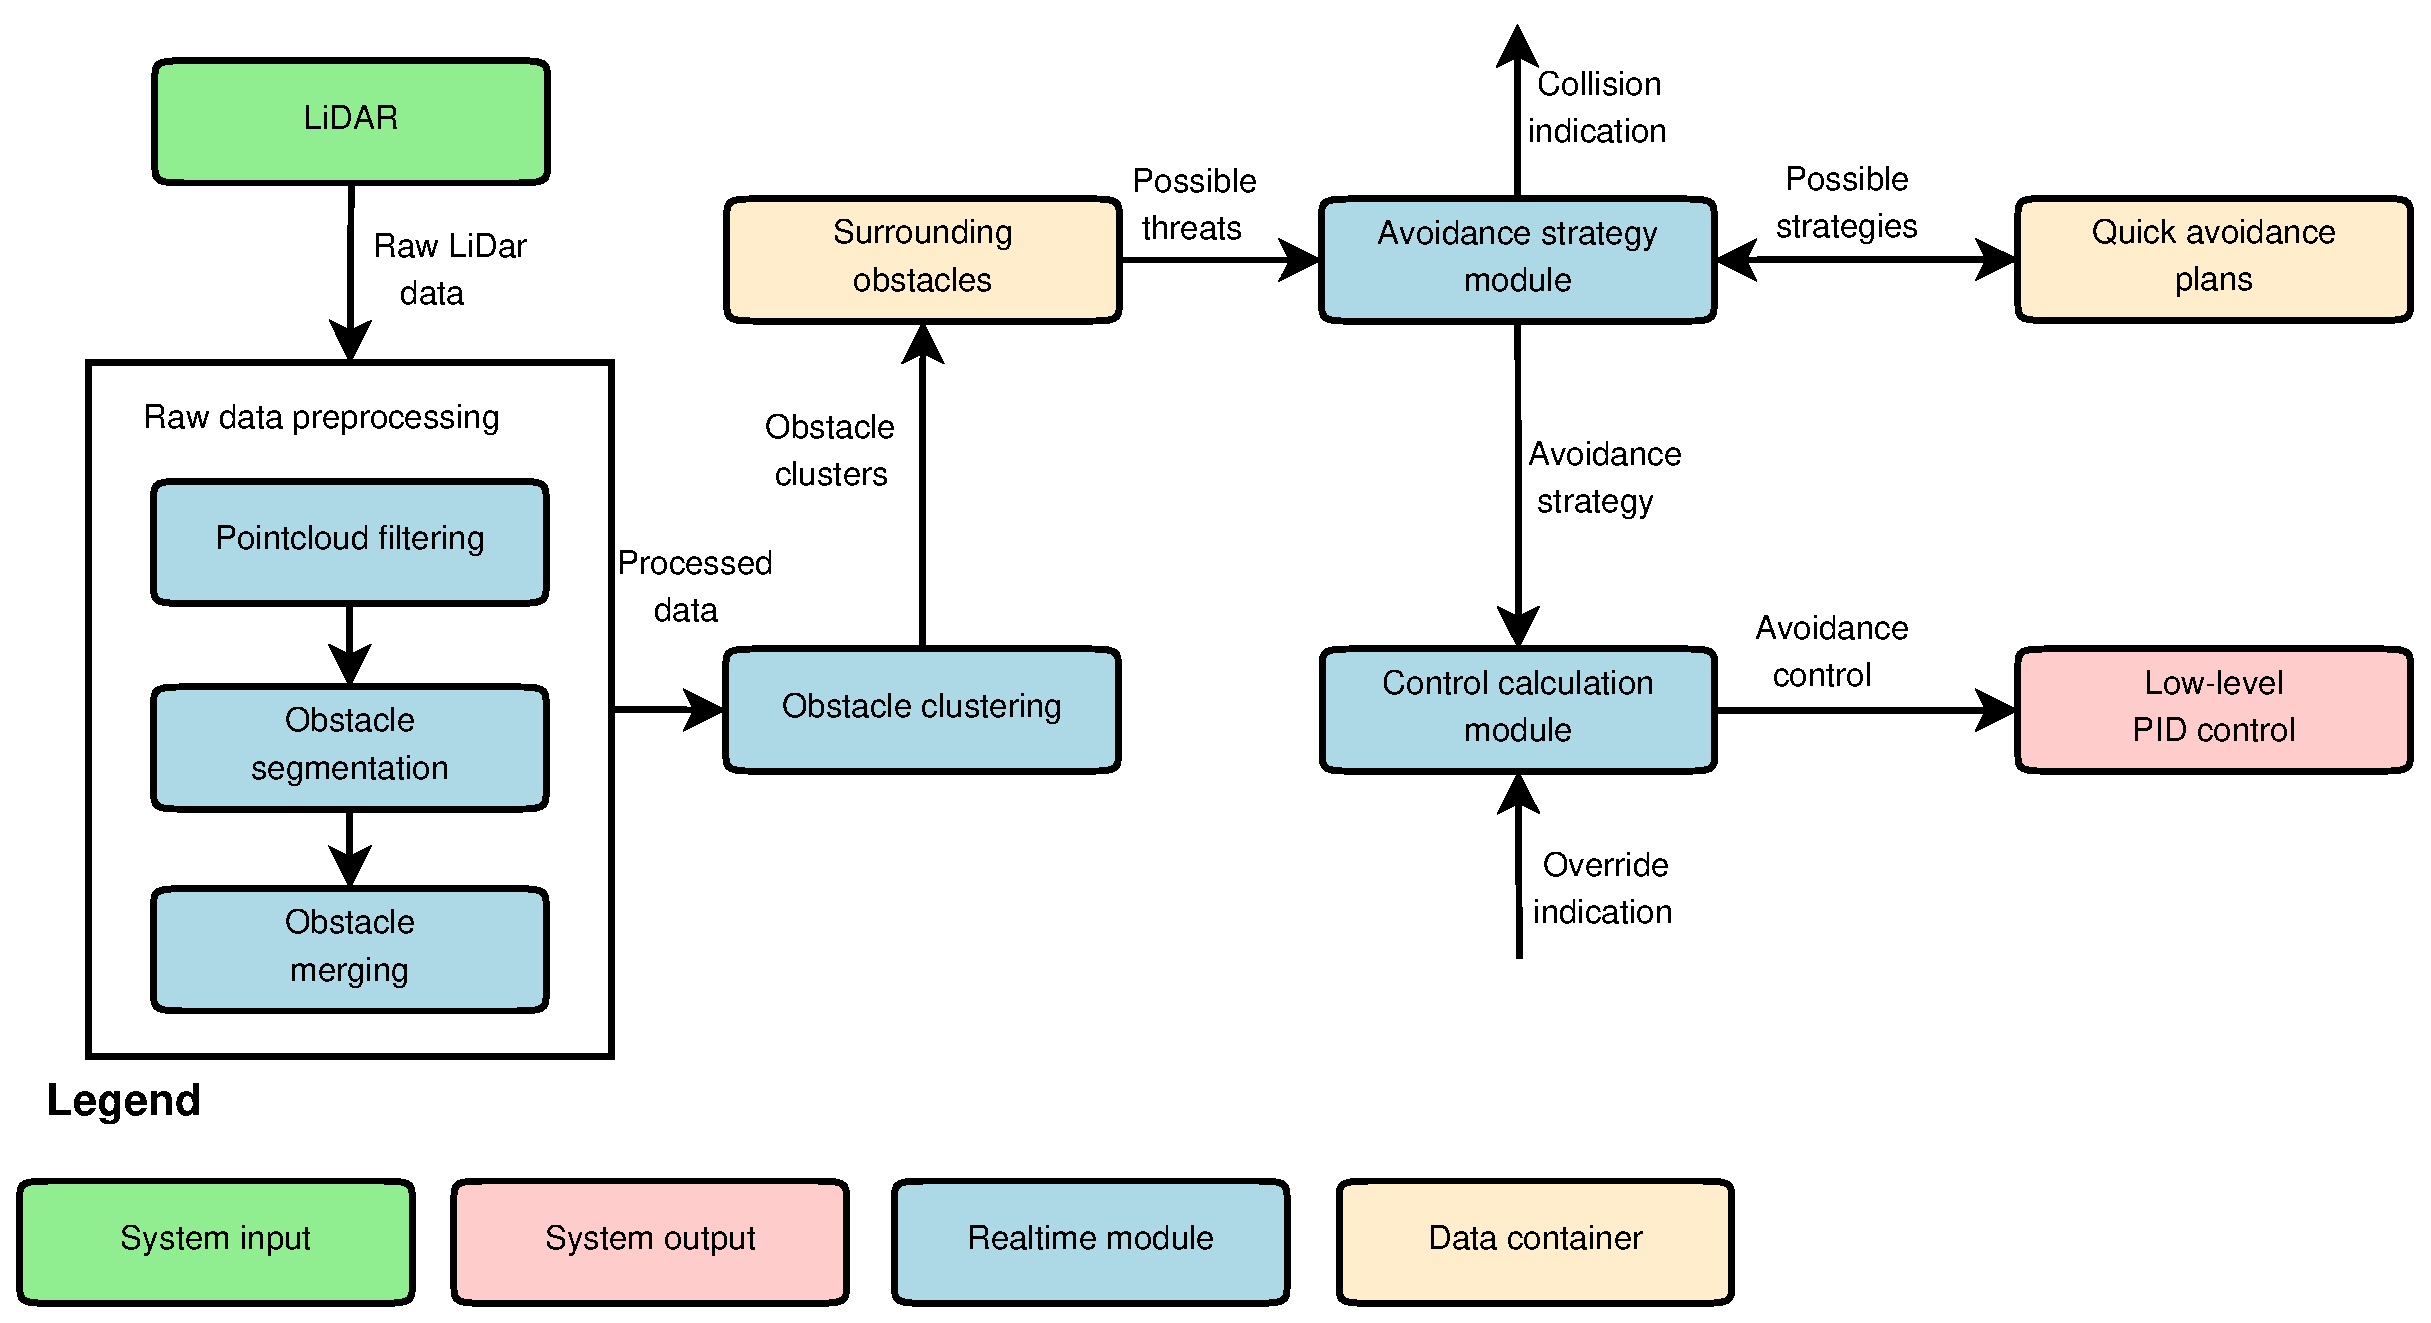
\includegraphics[width=\textwidth]{Pics/EmergencyControlModule.eps}
    \caption{Emergency control module scheme}
    \label{fig:EmergencyControlModule}
\end{figure}

\subsubsection{Raw data processing}
\begin{enumerate}[1.]
	\item Pointcloud filtering
	\item Obstacle segmentation
	\item Obstacle merging
\end{enumerate}
\begin{enumerate}[]
	\item \textbf{Role}
	    \begin{enumerate}[]
		    \item TODO
		\end{enumerate}
	\item \textbf{Input:}
	    \begin{enumerate}[1.]
		\item TODO
		\end{enumerate}	
	\item \textbf{Output:}
	    \begin{enumerate}[1.]
		\item TODO
		\end{enumerate}
\end{enumerate}

\subsubsection{Obstacle clustering}
TODO
\begin{enumerate}[]
	\item \textbf{Role}
	    \begin{enumerate}[]
		    \item TODO
		\end{enumerate}
	\item \textbf{Input:}
	    \begin{enumerate}[1.]
		\item TODO
		\end{enumerate}	
	\item \textbf{Output:}
	    \begin{enumerate}[1.]
		\item TODO
		\end{enumerate}
\end{enumerate}

\subsubsection{Surroundings obstacles}
TODO
\begin{enumerate}[]
	\item \textbf{Role}
	    \begin{enumerate}[]
		    \item TODO
		\end{enumerate}
	\item \textbf{Input:}
	    \begin{enumerate}[1.]
		\item TODO
		\end{enumerate}	
	\item \textbf{Output:}
	    \begin{enumerate}[1.]
		\item TODO
		\end{enumerate}
\end{enumerate}

\subsubsection{Quick avoidance plans}
TODO
\begin{enumerate}[]
	\item \textbf{Role}
	    \begin{enumerate}[]
		    \item TODO
		\end{enumerate}
	\item \textbf{Input:}
	    \begin{enumerate}[1.]
		\item TODO
		\end{enumerate}	
	\item \textbf{Output:}
	    \begin{enumerate}[1.]
		\item TODO
		\end{enumerate}
\end{enumerate}

\subsubsection{Avoidance strategy module}
TODO
\begin{enumerate}[]
	\item \textbf{Role}
	    \begin{enumerate}[]
		    \item TODO
		\end{enumerate}
	\item \textbf{Input:}
	    \begin{enumerate}[1.]
		\item TODO
		\end{enumerate}	
	\item \textbf{Output:}
	    \begin{enumerate}[1.]
		\item TODO
		\end{enumerate}
\end{enumerate}

\subsubsection{Control calculation module}
TODO
\begin{enumerate}[]
	\item \textbf{Role}
	    \begin{enumerate}[]
		    \item TODO
		\end{enumerate}
	\item \textbf{Input:}
	    \begin{enumerate}[1.]
		\item TODO
		\end{enumerate}	
	\item \textbf{Output:}
	    \begin{enumerate}[1.]
		\item TODO
		\end{enumerate}
\end{enumerate}

\subsubsection{Communication interfaces}
TODO
\begin{enumerate}[1.]
    \item Collision indication
	\item Override indication
\end{enumerate}
